\chapter{Methods}

% ============================================ OVERVIEW ===============================================
\section {Overview}
\label{sec:overview}

\subsection{The COSFIRE Approach}
COSFIRE filters are effective for keypoint detection and for pattern recognition. They are trainable because they can be configured with any given prototype patterns. They are constructed by a configuration process which automatically analyses the dominant orientations and their mutual spatial arrangement of a given prototype pattern of interest \cite{Azzopardi_Petkov_2012}. Gabor filters are used to detect the dominant orientations. The response of a COSFIRE filter is computed as the weighted geometric mean of the involved Gabor filter responses. This means that a response is only achieved when all the concerned contour parts are present \cite{Azzopardi_Petkov_2012}.


\subsection{Evaluation}
The research method applied in this project is quantitative. This also includes data analysis and hypothesis testing. Through the application of COSFIRE filters and classification techniques on publicly available data sets the performance measurements are computed in the form of true positives and false positive rates which are used to derive accuracy, precision and recall rates. The data sets that are used have different levels of complexity due to noise, deformation, rotation and scaling. The way we evaluate COSFIRE filters for these data set is as follows. \\

First, in a configuration stage, the COSFIRE filter is applied for each symbol model in the data set to create a collection of COSFIRE operators. Subsequently, with the attained COSFIRE operators, a shape descriptor is formed which takes an image as input and creates a feature vector representing the input image according to the operators from the configuration phase. Finally we use the resulting feature vectors to classify test images. \\


% ===================================================COSFIRE OVERVIEW================================================
\section {COSFIRE Method}
\label{sec:cosfiremethod}

\subsection{Overview}
COSFIRE filters are configured by first specifying a point of interest. In Fig.\ref{fig:ProtoTypePatternExample} a model symbol is used as an input image from which a local contour pattern is chosen as a prototype, encircled in Fig. \ref{fig:examplesymbol}. This prototype pattern is used to automatically configure a COSFIRE filter that responds to similar patterns.\\

\begin{figure*}[h]
        \centering
        \begin{subfigure}[b]{0.36\textwidth}
                \centering
                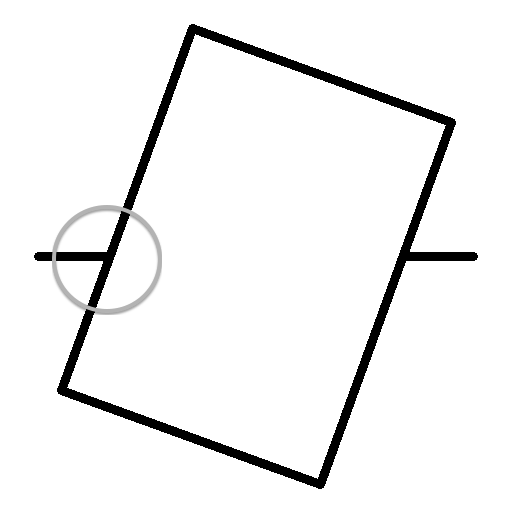
\includegraphics[width=0.6\textwidth]{figures/Method/ModelPointOfInterest.png}
                \caption{}
                \label{fig:examplesymbol}
        \end{subfigure}
        \begin{subfigure}[b]{0.36\textwidth}
                \centering
                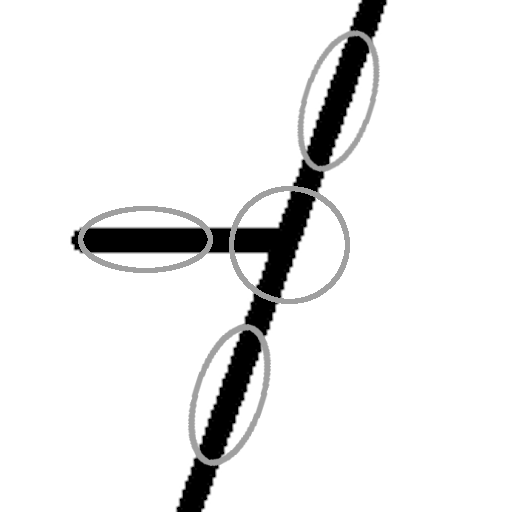
\includegraphics[width=0.6\textwidth]{figures/Method/DominantOrientationsAroundPointOfInterest.png}
                \caption{}
                \label{fig:modelsymbolvertex}
        \end{subfigure}
        \caption[Example of a prototype pattern]{(a) A model symbol (of size 512x512 pixels), of which one bifurcation (encircled) is used as a prototype pattern. (b) The enlarged prototype pattern where the dominant orientations around the point of interest are marked by 3 ellipses.}
        \label{fig:ProtoTypePatternExample}
\end{figure*}

The three ellipses shown in Fig. \ref{fig:modelsymbolvertex} around the encircled bifurcation illustrate the dominant orientations in the spatial arrangement around the chosen point of interest. These dominant orientations are detected by using symmetric Gabor filters. The selection of Gabor filter responses depends on the analysis of the local prototype pattern. The encircled bifurcation represents the overlapping support of a group of Gabor filters.

During the application of the COSFIRE method, different Gabor filter responses are taken at different locations around a point by shifting the responses of these Gabor filters by different vectors. The type of Gabor filters, the locations at which we take their responses, and the shifting vectors are determined in a automatic configuration stage. Then the shifted responses are used for the pixel-wise evaluation of a multivariate function which ultimately produces the COSFIRE filter's output.The COSFIRE filter achieves a response only when presented with the same or similar spatial arrangement of lines with similar orientations and thicknesses to the prototype.



% ======================================================GABOR FILTERS================================================
\subsection{Using Gabor filters to Detect Orientations}
The dominant orientations around a specified point of interest are detected by using symmetric two-dimensional (2D) Gabor filters. A 2D Gabor filter is defined as the product of an elliptical Gaussian and a sinusoid plane wave and is defined as follows:

\begin{equation}
   g(x,y;\lambda,\theta,\psi,\delta,\gamma) = \exp(-\frac{x'^2+\gamma^2y'^2}{2\delta^2}) \exp(2\pi \frac{x'}{\lambda}+\psi)
\end{equation}

\begin{equation}
x' = x \cos(\theta)+y\sin(\theta)
\end{equation}

\begin{equation}
y' = -x \sin(\theta)+y\cos(\theta)
\end{equation}

The $\lambda$ parameter, whose value is specified in pixels, represents the wavelength of the cosine factor, therefore the preferred wavelength of the filter. The $\theta$ parameter, who's value is specified in degrees, represents the orientation. The $\psi$ parameter represents the phase offset of the cosine factor whose values, from 0 to 180, determine whether the Gabor function is symmetric or not. A symmetric Gabor function is produced by setting the $\psi$,phase offset, parameter value to 0$^{\circ}$ or 180$^{\circ}$.\\

In this dissertation, the response of a symmetric Gabor filter at a given location (x,y) that is selective for a bar structure of orientation $\theta^{\circ}$ and thickness $2\lambda$ is denoted by $g_{\lambda,\theta}(x,y)$. The response represents the detection of a contour part within the image of wavelength $\lambda$ and of orientation $\theta^{\circ}$. Fig.\ref{fig:ModelGabor} shows two examples of Gabor filters, of the same wavelength but with different orientations being applied to a symbol model image. \\

\begin{figure*}[h]
        \centering
        \begin{subfigure}[b]{0.3\textwidth}
                \centering
                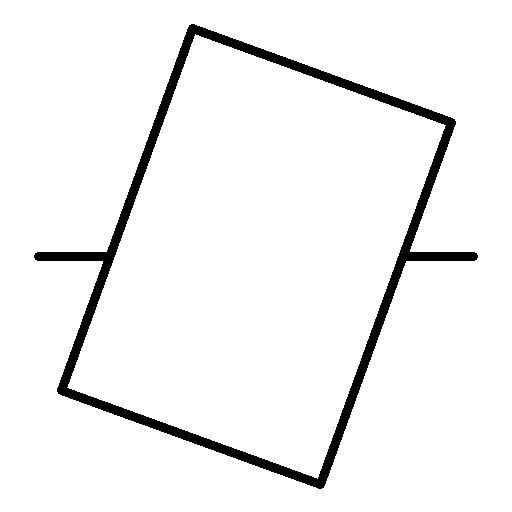
\includegraphics[width=0.8\textwidth]{figures/Method/ModelSymbol1.png}
                \caption{}
                \label{fig:examplesymbol2}
        \end{subfigure}
        \begin{subfigure}[b]{0.3\textwidth}
                \centering
                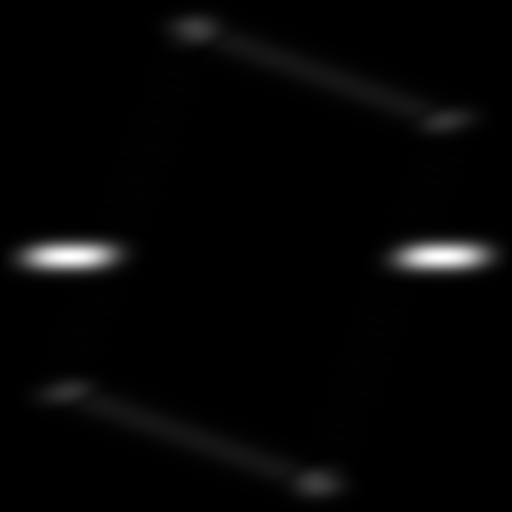
\includegraphics[width=0.8\textwidth]{figures/Method/gabor_15_95.png}
                \caption{}
                \label{fig:gab1090}
        \end{subfigure}
        \begin{subfigure}[b]{0.3\textwidth}
                \centering
                
\includegraphics[width=0.8\textwidth]{figures/Method/gabor1_15_160.png}
                \caption{}
                \label{fig:gab10130}
        \end{subfigure} 
        \caption[Gabor filter applications]{(b) A Gabor filter when applied to a (a) model symbol with $\lambda = 15 $ and $\theta = 90^{\circ}$. (c) The response of a Gabor filter when applied to a (a) model symbol with $\lambda = 15 $ and $\theta = 160^{\circ}$.}
        \label{fig:ModelGabor}
\end{figure*}


We then threshold the Gabor responses in order to eliminate undesirable responses to some noise or to undesirable responses around the contour parts. This threshold, $t1 = (0 \leq t1 \leq 1)$, is a fraction of the maximum response of $g_{\lambda,\theta}(x,y)$ across all combinations of values $(\lambda,\theta)$ and all possible positions within the image $(x,y)$. The threshold responses are then denoted by $| g_{\lambda,\theta}(x,y)|_{t1}$. The value of the $t1$ threshold depends on the contrast the image contains. Ultimately, this threshold parameter controls the level at which a Gabor filter's response recognises the presence of a contour part. For our experiments we found that a value of t1 = 0.1 is sufficient.\\


% =============================================COSFIRE CONFIGURATION================================================
\subsection{Configuration}
As input, COSFIRE filters use the responses of specific Gabor filters. Each of these Gabor filters responses represent a contour part in an image. Each response is denoted as a set of four parameter values, $( \lambda_{i}, \theta_{i}, \rho_{i}, \phi_{i} )$. The width of the detected contour part is represented by $\lambda_{i}$. The orientation of the same contour part is represented by $\theta_{i}$. Finally its location is represented by polar coordinates $\rho_{i}$ and $\phi_{i}$ with respect to the point of interest.\\

The parameter values of these contour parts are obtained as follows. A circle of radius $\rho$ is placed around the point of interest. Along this circle we consider the responses of a bank of Gabor filters. From all those Gabor filters' responses we only take those that have the maximum response across all filters, that is across all combinations of $(\lambda, \theta)$. These are chosen to be the dominant orientations around the point of interest. We then determine the polar coordinates of the chosen points, in respect to the center of the COSFIRE filter. \\

\begin{figure*}[h]
        \centering
        \begin{subfigure}[b]{0.3\textwidth}
                \centering
                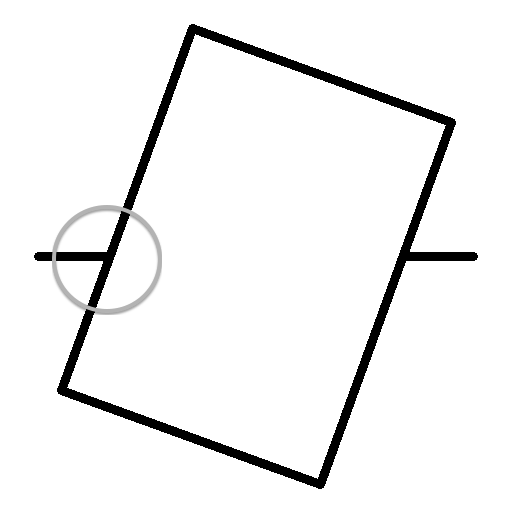
\includegraphics[width=0.8\textwidth]{figures/Method/ModelPointOfInterest.png}
                \caption{}
                \label{fig:modelsymbol}
        \end{subfigure}
        \begin{subfigure}[b]{0.3\textwidth}
                \centering
                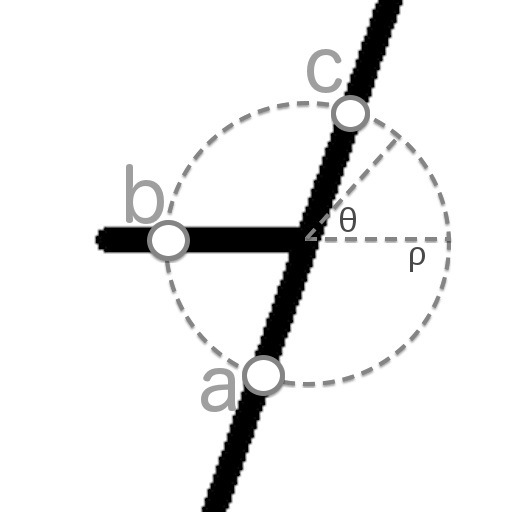
\includegraphics[width=0.8\textwidth]{figures/Method/actualConfiguration.jpg}
                \caption{}
                \label{fig:cosfireconf}
        \end{subfigure}
        \caption[Example configuration of a COSFIRE filter]{(a) A circle of radius $\rho$ is placed around a point of interest. (b) The points marked by labels a, b, and c represent the locations at which the Gabor filters achieve local maxima responses.}
        \label{fig:COSFIREConfigurationExample}
\end{figure*}


Fig. \ref{fig:COSFIREConfigurationExample} shows an example configuration of a COSFIRE filter by with a circle around the point of interest in a symbol model image. For each location ($\rho,\phi$) we then consider all the combinations of $(\lambda, \theta)$ for which the corresponding Gabor filter response, $_{g\lambda,\theta}(x,y)$, is greater than a fraction,$t_{2}=0.75$, of the maximum response across all the combinations of $\lambda$ and $\theta$.
For each value of $\theta$ that satisfies the condition above, we consider a single value of $\lambda$ from the maximum of all responses. For each unique pair of ($\lambda, \theta$), for location ($\rho,\phi$) we then obtain a tuple $( \lambda_{i}, \theta_{i}, \rho_{i}, \phi_{i} )$. \\

More than one tuple can also be formed in the same location. Therefore, we express the set of parameter value combinations as $S_f= \begin{Bmatrix}( \lambda_{i}, \theta_{i}, \rho_{i}, \phi_{i} ) | i=1...n_{f} \end{Bmatrix}$. The $f$ subscript stands for the local prototype pattern around the specified point of interest. Fig. \ref{fig:COSFIREConfigurationExample2} is an example of the resultant configured operator from Fig. \ref{fig:COSFIREConfigurationExample}.

\begin{figure*}[h]
        \centering
        \begin{subfigure}[b]{0.3\textwidth}
                \centering
                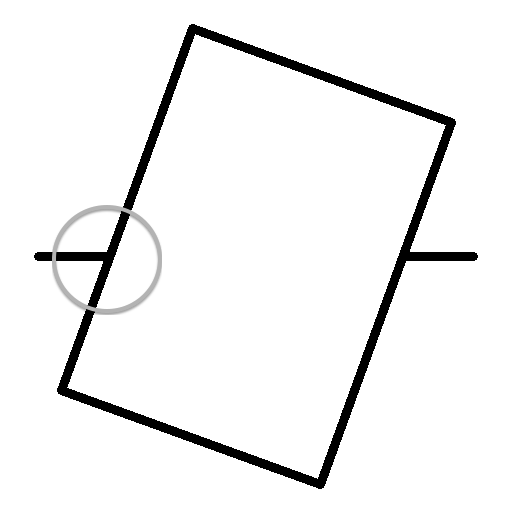
\includegraphics[width=0.8\textwidth]{figures/Method/ModelPointOfInterest.png}
                \caption{}
                \label{fig:modelsymbol}
        \end{subfigure}
        \begin{subfigure}[b]{0.3\textwidth}
                \centering
                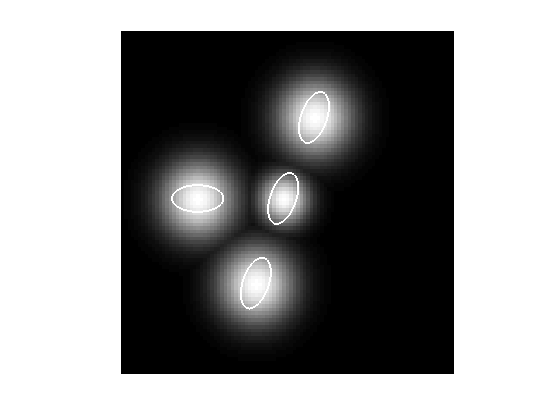
\includegraphics[width=0.8\textwidth]{figures/Method/COSFIREOPerator.png}
                \caption{}
                \label{fig:cosfireconf}
        \end{subfigure}
        \caption[Example of a COSFIRE operator for a prototype pattern.]{(b) A COSFIRE operator is configured upon selecting (a) a prototype pattern where $\rho = 14$ }
        \label{fig:COSFIREConfigurationExample2}
\end{figure*}

The following shows the collection of tuples,$S_{f}$, returned by the COSFIRE operator shown in Fig.\ref{fig:COSFIREConfigurationExample2}. These tuples are then used in the application of the COSFIRE filter.

\begin{equation}
  S_{f} = \begin{Bmatrix*} 
                  (\lambda_1 = 11.3137, & \theta_1 = 2.7925,    & \rho_1 = 0,  & \phi_1 = 0), \\
                  (\lambda_2 = 11.3137, & \theta_2 = 2.7925,    & \rho_2 = 14, &\phi_2 = 1.2043), \\
                  (\lambda_3 = 11.3137, & \theta_3 = 1.5708,    & \rho_3 = 14, &\phi_3 = 3.1416), \\
                  (\lambda_4 = 11.3137, & \theta_4 = 1.6581,    & \rho_4 = 14, &\phi_4 = 3.1416), \\
                  (\lambda_5 = 11.3137, & \theta_5 = 2.7925,    & \rho_5 = 14, &\phi_5 = 4.4157), \\
              \end{Bmatrix*}
\end{equation} \\

\subsection{Application of a COSFIRE Filter}
\subsubsection{Applying Gabor filters}
For each tuple $i$ in the configured set $S_f$ we apply a Gabor filter, to a test image, with the corresponding parameters $\lambda_i$ and $\theta_i$. A maximum response is achieved for a bar structure that has an orientation $\theta_i$ and thickness $2\lambda_i.$ 

\subsubsection{Blurring and Shifting of Gabor responses}
First, we blur the Gabor filter responses in order to allow for some tolerance in the position of their respective contour parts. \\

The blurring operation is defined as the computation of maximum value of the weighted thresholded responses of a Gabor filter. A Gaussian function, $G_{\sigma}(x,y)$, is used for weighting. The $\sigma$ parameter represents the standard deviation of the Gaussian function which is expressed as a linear function of distance $\rho$ from the center of the COSFIRE filter as shown in Eq. 1.5. where $\sigma_{0}$ and $\alpha$ are constants and the $\alpha$ parameter value determines the orientation tuning of the COSFIRE filter.

\begin{equation}
 \sigma = \sigma_{0}+\alpha\rho
\end{equation}
\label{eq:gStandardDeviation}

We then take the blurred Gabor filter responses and shift them to the filter's centre so they meet at the same position, the same position we consider the center of support of the concerned COSFIRE filter. Each response is shifted by a distance $\rho_{i}$ in the direction opposite of $\phi_{i}$. In polar coordinates the shift vector by which the Gabor filter responses are shifted is specified by $(\rho_{i},\phi_{i} + \pi)$ where as in cartesian coordinates it is specified as $(\Delta x_{i},\Delta y_{i})$ where $\Delta x_{i}=-\rho_{i} \cos(\phi_{i})$ and $\Delta y_{i}=-\rho_{i} \sin(\phi_{i})$. The blurred and shifted response of a Gabor filter, specified by the $i$-th tuple $( \lambda_{i}, \theta_{i}, \rho_{i}, \phi_{i} )$ in $S_{f}$, is denoted by $s_{( \lambda_{i}, \theta_{i}, \rho_{i}, \phi_{i} )}(x,y)$.

\begin{equation}
s_{( \lambda_{i}, \theta_{i}, \rho_{i}, \phi_{i} )}(x,y) = \underset{x',y'}{max} \begin{Bmatrix*} |g_{\lambda_{i}, \theta_{i}} (x-x'-\Delta x_{i},y-y'-\Delta y_{i})|_{t_{1}} G_{\sigma}(x',y') \end{Bmatrix*}
\end{equation}

\begin{equation}
-3\sigma \leq x,y \leq 3\sigma
\end{equation}



\subsubsection{Response of a COSFIRE filter}
The response of a COSFIRE filter, denoted by $r_{S_{f}}(x,y)$, is defined as the weighted geometric mean of all the thresholded blurred and shifted Gabor filter responses, denoted by $s_{\lambda_{i}, \theta_{i}, \rho_{i}, \phi_{i}} (x,y)$, that correspond to the contour parts defined in $S_{f}$: 


\begin{equation}
r_{S_{f}}(x,y) = \left|\left(\prod_{i=1}^{|S_{f}|} \left(s_{\lambda_{i}, \theta_{i}, \rho_{i}, \phi_{i}}(x,y)\right)^{\omega_{i}}\right)^{1/\sum_{i=1}^{|S_{f}|} \omega_{i}}\right|_{t_{3}}
\end{equation}

\begin{equation}
\omega_{i} = exp -\frac{\rho_{i}^2}{2\sigma'^2} , 0 \leq t_{3} \leq 1
\end{equation}

The $|.|_{t_{3}}$ stands for the thresholding the response at a fraction $t_{3}$ of its maximum across all image coordinates. COSFIRE filters can achieve invariance to rotation, scale, reflection and contrast inversion. We refer to \cite{Azzopardi_Petkov_2012} for the technical description of how invariance of COSFIRE filters is achieved


\section {Evaluation}
\label{sec:evaluation}
\subsection{Pre-Processing}
Each dataset's collection of test images varies according to some amount of deformation, noise or geometrical transformation. In order to aid the classification process a number of pre-processing steps were taken in order to clean/enhance the test images. As an initial step all test images are resized by a specific factor. 
Furthermore, test images which contain salt and pepper noise, such as noise E's, are de-noised using median filtering and degraded test images, such as Noise A's, are enhanced by the use of dilation. Other test images, such as Noise B's were thickened. Also with this thickening noise was included, therefore both median filtering and thinning were applied. The following are the pre-processing techniques which were applied in this evaluation.

\subsubsection{Re-sizing}
For efficiency reasons, prior to configuring COSFIRE filter/s we first resize the model by a factor of $0.5$, using bicubic interpolation, before being inputted into the configuration and training phases. The original model images are of size $(512 \times 512)$ pixels. By applying a resize factor of $0.5$, the images are resized to $(512(0.5) \times 512(0.5)) = (256 \times 256)$ pixels. This reduces the time in which the COSFIRE operator is applied to an image by half due to less information to process. No pre-processing was done on the test images.

\subsubsection{De-noising by median filtering}
Datasets such as the Noise E contain "salt and pepper" noise. Therefore before running an experiment using those datasets some pre-processing is required in order to reduce noise. De-noising is done through the use of median filtering. A median filter considers each pixel in the image sequentially and analyses the surrounding pixels. The value of the considered pixel is replaced with the median of the values of the surrounding pixels \cite{medianFiltering}. This reduces the noise from the image as shown in Fig. \ref{fig:mf} .

\begin{figure*}[h]
        \centering
        \begin{subfigure}[b]{0.3\textwidth}
                \centering
                \fbox{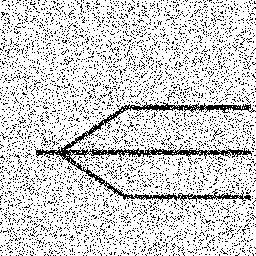
\includegraphics[width=0.8\textwidth]{figures/Method/image04.png}}
                \caption{}
                \label{fig:modelsymbol}
        \end{subfigure}
        \begin{subfigure}[b]{0.3\textwidth}
                \centering
                \fbox{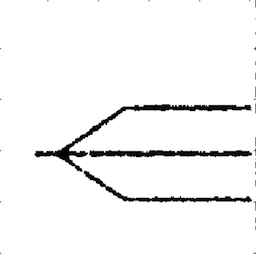
\includegraphics[width=0.8\textwidth]{figures/Method/untitled.png}}
                \caption{}
                \label{fig:mf123}
        \end{subfigure}
        \caption[Example output of median filtering.]{(a) A symbol with salt and pepper noise is (b) processed through the use of median filtering}
        \label{fig:mf}
\end{figure*}

\vspace{100mm}

\subsubsection{Dilation}
Some datasets, such as Noise A, have degraded test images. Before classifying such as test images an other pre-processing step that is implemented is morphological dilation. 
The effect of morphological dilation is to gradually enlarge the boundaries of specific regions of foreground pixels. Therefore these regions grow in size while holes or gaps within the symbol become smaller, thus enhancing the image. In order to do this a structuring element is used which determines the dilation effect on the test image \cite{dilation}. Fig \ref{fig:dilate} shows an example.

\begin{figure*}[h]
        \centering
        \begin{subfigure}[b]{0.3\textwidth}
                \centering
                \fbox{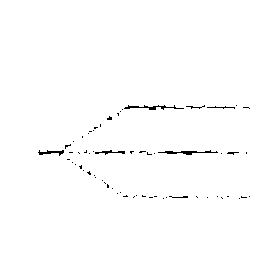
\includegraphics[width=0.8\textwidth]{figures/Method/image11.png}}
                \caption{}
                \label{fig:modelsymbol}
        \end{subfigure}
        \begin{subfigure}[b]{0.3\textwidth}
                \centering
                \fbox{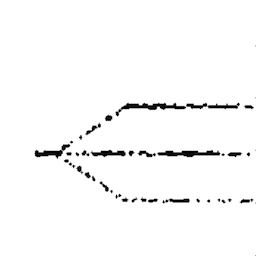
\includegraphics[width=0.8\textwidth]{figures/Method/image11Dilate.png}}
                \caption{}
                \label{fig:mf123}
        \end{subfigure}
        \caption[Example output of dilation.]{(a) A symbol of degraded quality (b) is processed using morphological dilation}
        \label{fig:dilate}
\end{figure*}

\subsubsection{Thinning}
Thinning is an other morphological operator which removes pixels so that an object shrinks to a minimal stroke. Like dilation, thinning relies on a structuring element \cite{thinning}. Datasets, such as noise B, contain test images which have their lines' thickened. Further more, the process of thickening the symbol's geometric parts adds noise around the edges as well. This is countered by doing the following. Like dilation, thinning relies on a structuring element \cite{thinning}. In this case, we use a structuring element of line form. Twelve different line structuring elements are created with different orientations. These orientations are applied to the test image and the outputs for each are then superimposed. Subsequently skeletonisation and dilation using a disc structuring elements are applied. A median filter is also applied, in order to remove the noise around the edges, and thinning. Fig \ref{fig:thickness} shows an example.

\begin{figure*}[h]
        \centering
        \begin{subfigure}[b]{0.3\textwidth}
                \centering
                \fbox{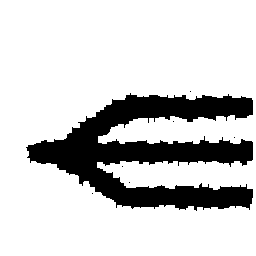
\includegraphics[width=0.8\textwidth]{figures/Method/image03.png}}
                \caption{}
                \label{fig:modelsymbol}
        \end{subfigure}
        \begin{subfigure}[b]{0.3\textwidth}
                \centering
                \fbox{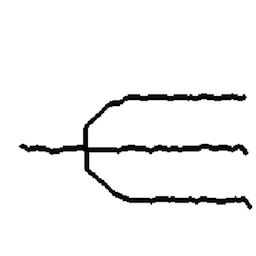
\includegraphics[width=0.8\textwidth]{figures/Method/image03Thinning.png}}
                \caption{}
                \label{fig:mf123}
        \end{subfigure}
        \caption[Example output of thinning.]{(a) A symbol of thickened quality (b) is processed using median filtering and thinning}
        \label{fig:thickness}
\end{figure*}

\subsection{Forming a Shape Descriptor}
\label{sec:descriptor}

In the configuration process of COSFIRE filters, features of interest are chosen by specifying a point or a collection of points within the model symbol. The system automatically analyses those points and extracts information about the dominant orientations and their mutual spatial arrangement according to the list of concentric circles surrounding the point of interest. The number of concentric circles is not intrinsic to the method but rather to the complexity of the given prototype pattern of interest. These are the prototype patterns that the COSFIRE filter will learn to recognise in the testing images. \cite{Azzopardi_Petkov_2012}. \\

For the purpose of electrical and architectural symbol recognition, a COSFIRE filter is configured for every model symbol in a given data set. These configurations were approached in two ways. In the first approach that was used in the first six experiments, was to select a single static point of interest which was placed in the middle of the model symbol. Fig. \ref{fig:COSFIREoperatorExample} shows a configuration, using the described single point approach.
%
\begin{figure*}[h]
        \centering
        \begin{subfigure}[b]{0.3\textwidth}
                \centering
                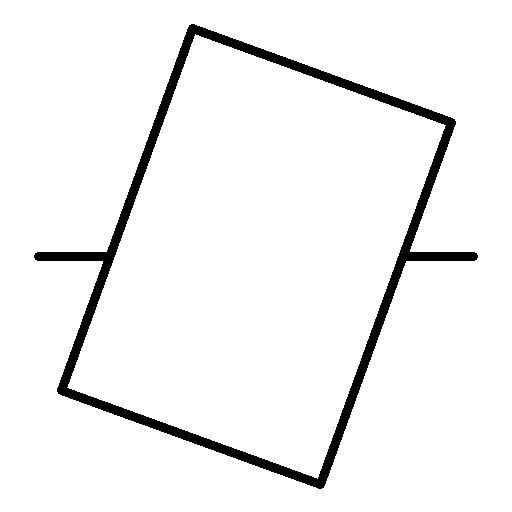
\includegraphics[width=0.8\textwidth]{figures/Method/ModelSymbol1.png}
                \caption{}
                \label{fig:modelsymbol}
        \end{subfigure}
        \begin{subfigure}[b]{0.3\textwidth}
                \centering
                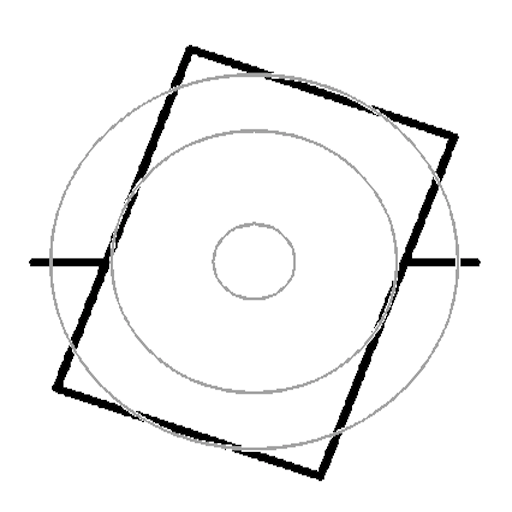
\includegraphics[width=0.8\textwidth]{figures/Method/ModelRhoConfiguration.png}
                \caption{}
                \label{fig:cosfireconf}
        \end{subfigure}
        \caption[Configuration of a COSFIRE filter using single point approach]{A COSFIRE filter is configured by first placing (b) the point of interest at the centre of the (a) model symbol}
        \label{fig:COSFIREoperatorExample}
\end{figure*}

The resulting COSFIRE filters are used to build a shape descriptor as follows. The created COSFIRE operators are applied to each symbol model. Each COSFIRE operator achieves a response for every location in the given image. From this response image, we choose the one that has the maximum value. This means that a symbol model image is described by a vector of values with a size that is equivalent to the number of COSFIRE filters used.\\

Fig. \ref{fig:shapedescriptor} shows an example of the result attained when the model symbols are processed by the shape descriptor. In this example there are 17 models images and 1 operator is applied to each model image. Each model image is therefore represented by a feature vector of 17 maximum values. The diagonal values in this descriptor have the highest responses. These values correspond to the model image being applied to it's corresponding COSFIRE operator.\\

\begin{figure*}[h]
    \centering
    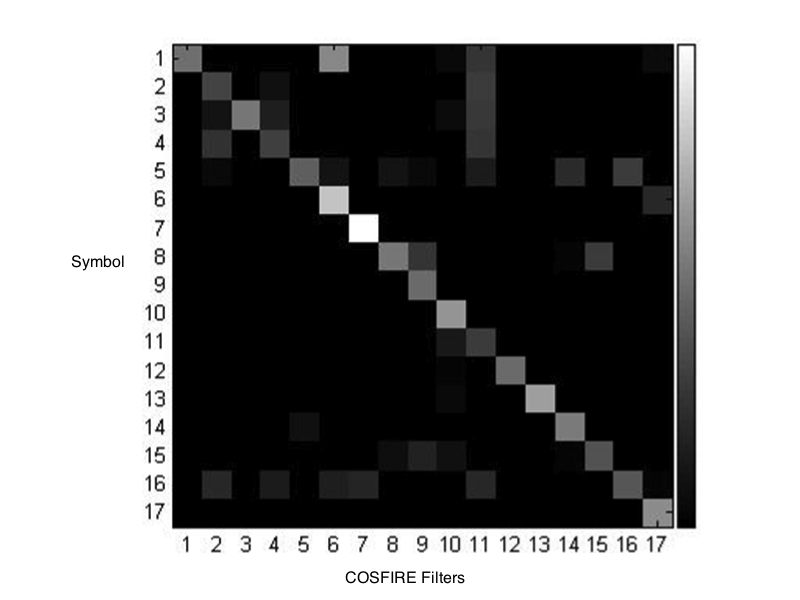
\includegraphics[totalheight=0.5\textheight, keepaspectratio]{figures/Method/ShapeDescriptor2.png}
    % \rule{.8\textwidth}{.8\textheight}{figures/ProjectPlan.jpg}
    \caption[Example of the feature vectors  for each model created by a shape descriptor]{A row {\em i} represents the feature vector of a symbol model composed of the maximum responses of COSFIRE filters. Element {\em j} of a feature vector {\em i} is the maximum response of a COSFIRE filter which is configured by model symbol {\em j}}
    \label{fig:shapedescriptor}
  \end{figure*}

Although the single point approach towards configuring filters produces good results in the first few datasets, a problem is introduced concerning the list of concentric circles used. Using the same list of concentric circles for all the datasets means that for some model symbols no dominant orientations could be detected.This resulted in test symbols not being properly recognised. An example is shown in Fig. \ref{fig:COSFIREoperatorErrorExample}.\\

\begin{figure*}[h]
        \centering
        \begin{subfigure}[b]{0.3\textwidth}
                \centering
                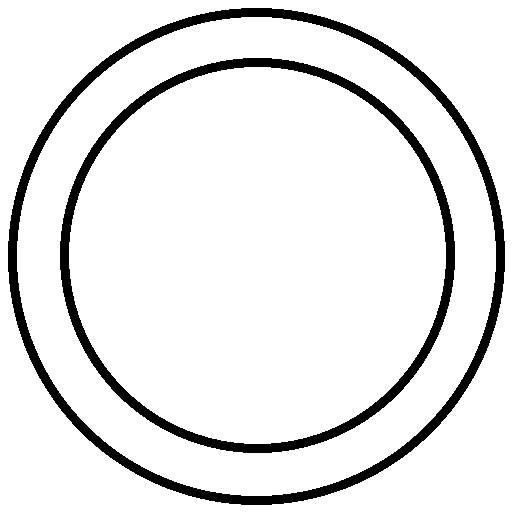
\includegraphics[width=0.6\textwidth]{figures/Method/ModelSymbol2.png}
                \caption{Model Symbol}
                \label{fig:modelsymbol}
        \end{subfigure}
        \begin{subfigure}[b]{0.3\textwidth}
                \centering
                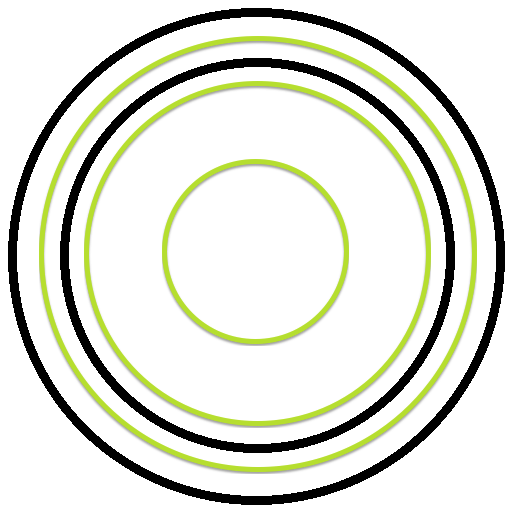
\includegraphics[width=0.6\textwidth]{figures/Method/CosfireOperatorSinglePointApproachError.png}
                \caption{COSFIRE Operator}
                \label{fig:cosfireoperator}
        \end{subfigure}
        \caption[Example of an incorrect configuration due to rho list ]{(b) Inappropriate selection of concentric circles around the center of (a) a specific model symbol. Here we use the same three concentric circles used in the previous example.}
        \label{fig:COSFIREoperatorErrorExample}
\end{figure*}
%%
In order to address this issue, an alternative approach is taken in selecting points of interest. The list of concentric circles is set to three and three points of interest are placed randomly in the symbol model image. Each of these points hold the same list of concentric circles. Doing so ensures that each model symbol has a unique set of detected contour parts. An example of this approach is shown in Fig. \ref{fig:3PointCOSFIREoperatorExample}.

\begin{figure*}[h]
        \centering
        \begin{subfigure}[b]{0.4\textwidth}
                \centering
                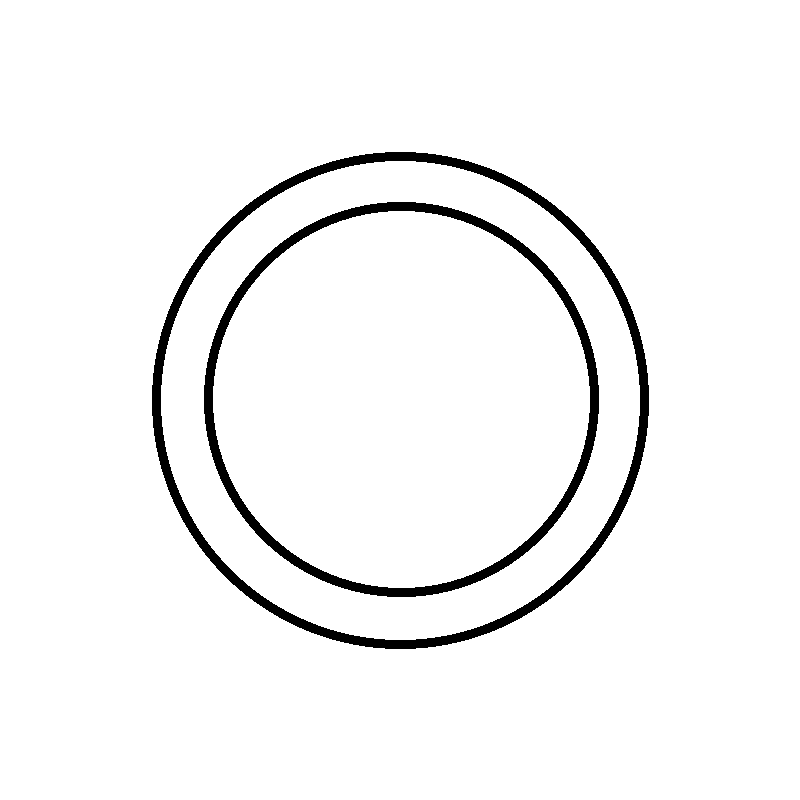
\includegraphics[width=0.8\textwidth]{figures/Method/ModelSymbol2_2.png}
                \caption{Model Symbol}
                \label{fig:modelsymbol}
        \end{subfigure}
        \begin{subfigure}[b]{0.4\textwidth}
                \centering
                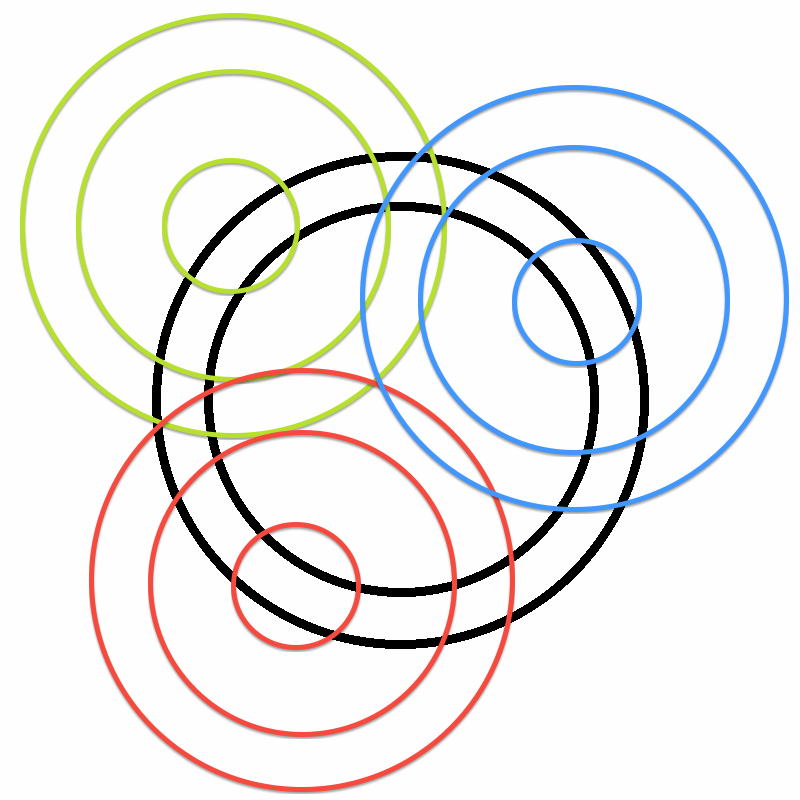
\includegraphics[width=0.8\textwidth]{figures/Method/CosfireOperatorThreePointApproach.png}
                \caption{COSFIRE Operator}
                \label{fig:cosfireoperator}
        \end{subfigure}
        \caption[An example of a 3-point approach in configuring COSFIRE filters.]{(b) Three COSFIRE filters are being configured for the symbol (a). The concentric circles for each point of interest are shown in different colours.}
        \label{fig:3PointCOSFIREoperatorExample}
\end{figure*}
\vspace{100mm}
This approach is driven by three parameters $\eta$, $\beta$, and $\varsigma$. The $\eta$ parameter value determines the number of points of interest placed in the model image. The $\beta$ parameter value determines the minimum number of tuples that should be attained from the point of interest's surrounding spatial arrangement. The $\varsigma$ parameter value determines the number of unique orientations that should be detected. This means that $\eta=3$ operators will be applied for each symbol mode. These operators should have a minimum of $\beta = 5$ tuples each with at least $\varsigma = 2$ unique orientations. \\

As a result of using the three point approach we have available a set of COSFIRE operators with a cardinality of three times the size of the total number of symbol model images available. Therefore for a dataset of $k$ model images, the configuration results in $3k$ distinct COSFIRE filter operators.
%[--!--]

%%============================================CLASSIFICATION===============================================
\subsection{Classification}
\label{sec:classify}
Classification refers to the problem of identifying, the set/s sets of categories/classes, certain objects or patterns belong to. In this thesis, this problem is tackled by trying to relate a test image to a specific symbol model by recognising contour parts which are similar in both the model image and the test image. This is done by using the feature vectors which represent both images.

\subsubsection{Feature Vectors}
Inputting each of the Model images into the shape descriptor, described in sub section \ref{sec:descriptor}, it creates a feature vector for each. This means that if there are 150 models in the data set and 3 operators are applied for each model 150 different feature vectors are created with 450 elements each. 

\subsubsection{Normalisation}
Prior to classification of the test images, normalisation is applied on both the training set of feature vectors and the testing set of feature vectors. This is done so that the test image and it's corresponding model image are rendered more comparable thus aiding the classification process. Normalisation is done using Z-Normalisation also known as zero-mean normalisation. This normalisation technique transforms the distribution of pixel values into a standard normal distribution. \\

For each 450 elements in the feature vector, the mean, $\mu_{x}$, and the standard deviation, $\sigma_{x}$, are computed. The configuration feature vectors are then normalised by subtracting the mean and diving the standard deviation. The same is done for the feature vectors which are extracted from the testing images. The following is how a normalised value is obtained using z-score normalisation \cite{zscore}:

\begin{equation}
 NormalisedValue = \frac{v-\mu_{x}}{\sigma_{x}}
\end{equation}
\label{eq:gStandardDeviation}


\subsubsection{K-nearest neighbour algorithm}
The K-nearest neighbour algorithm (K-nn), known to be amongst the top 10 data mining algorithms \cite{Wu_2007}, is a versatile technique who's application range from vision to computational geometry \cite{knn_online}. It has been used for the classification of objects or patterns according to the closest training examples available. Before using the Knn algorithm, some prerequisite steps need to be taken. The first step is to ensure that the data is in a feature space. This data can be both single scalars or even multidimensional vectors \cite{knn_online}. The second step is to define a constant $K$. \\

The constant $K$ is a user defined value. It is the number of instances / neighbours the algorithm allows to influence the classification \cite{knn_online}. Since the test symbol needs to be assigned to the class of its nearest neighbour, the constant $k$ is set to $k=1$. An other important step is to determine which distance metric to use. In order to classify the test image's feature vector to the nearest feature vector from the models a distance metric needs to be used. Since both the models and the test images are represented by feature vectors made of $n$ number of elements, the distance metric used in this classification process is Euclidean distance. Euclidean distance is defined as follows where $M$ is the feature vector for the model image and $T$ is the feature vector for the test image \cite{euclidean_online}. 

\begin{equation}
    d(M,T) = \sqrt{\sum_{i=1}^{n} (M_{i}-T)^2}
\end{equation}

Therefore classification is achieved by computing the Euclidean distance between the test image feature vector to each training feature vector in the shape descriptor. A test vector is then classified to the symbol for which the Euclidean distance is the smallest, therefore the most similar. An illustration of the Knn algorithm is shown in Fig. \ref{fig:knnexample}.


\begin{figure*}[h]
    \centering
    \includegraphics[totalheight=0.25\textheight, keepaspectratio]{figures/Method/knn.jpg}
    \caption[Example of K-nearest Neighbour algorithm]{An object (star) whose class is not known is being classified according to its nearest neighbours. Two examples are shown, where $k=3$ and $k=7$ \footnotemark.}
    \label{fig:knnexample}
\end{figure*}
\vspace{100mm}
\footnotetext[1]{Taken From \url{http://iopscience.iop.org/1742-5468/2010/11/P11015/fulltext/}}

.
\vspace{200mm}
\subsection{Evaluation Summary} 
Fig. \ref{fig:flowchart} shows a work flow of the whole evaluation process for this dissertation.
\begin{figure*}[h]
        \centering
        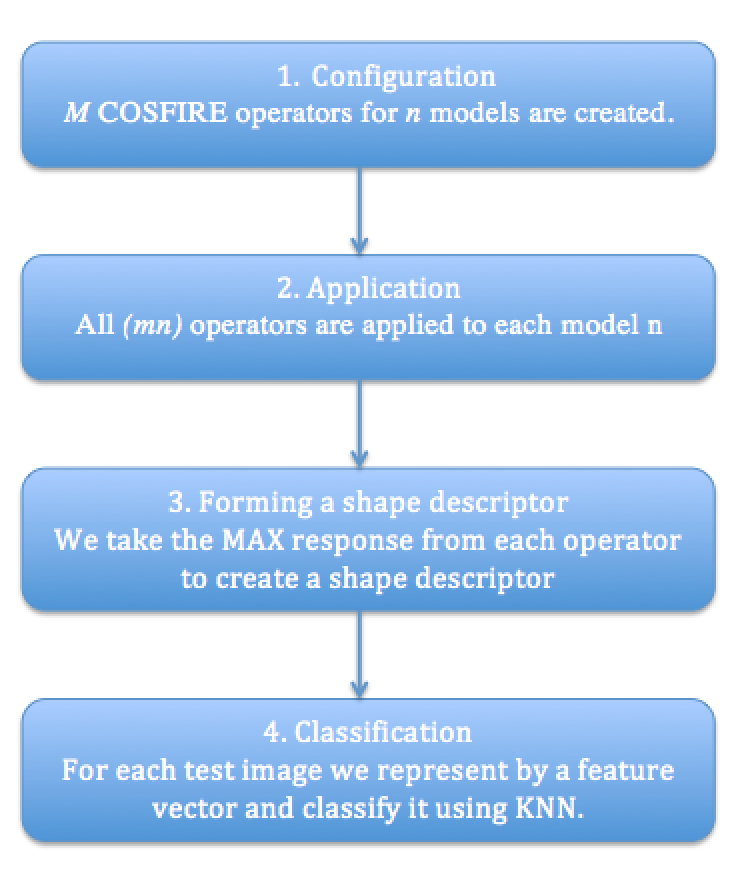
\includegraphics[width=0.8\textwidth]{figures/Method/workflow3.png}
        \caption[Evaluation flow chart]{(1) $M$ COSFIRE operators for $n$ model images are created. (2) All $(mn)$ operators are applied to each of the model images and (3) from those responses we take the maximum responses and create a feature vector for each model to form a shape descriptor. (4) We finally use the created shape descriptor to classify the images.  }
        \label{fig:flowchart}
\end{figure*}